% !TEX encoding = UTF-8 Unicode

\documentclass[a4paper]{article}

\usepackage{color}
\usepackage{url}
\usepackage[T2A]{fontenc} % enable Cyrillic fonts
\usepackage[utf8]{inputenc} % make weird characters work
\usepackage{graphicx}
\graphicspath{ {Slike/} }

\usepackage[english,serbian]{babel}
%\usepackage[english,serbianc]{babel} %ukljuciti babel sa ovim opcijama, umesto gornjim, ukoliko se koristi cirilica

\usepackage[unicode]{hyperref}
\hypersetup{colorlinks,citecolor=green,filecolor=green,linkcolor=blue,urlcolor=blue}


\begin{document}

\title{Optimizacija programa kroz različite pristupe Iterativnoj Kompilaciji\\ \small{Seminarski rad u okviru kursa\\Metodologija stručnog i naučnog rada\\ Matematički fakultet}}

\author{Filip Novović, Aleksandar Preočanin, Aleksandar Milosavljević\\ [!!!], preocanin.aleksandar@gmail.com, alemilosav@gmail.com }
\date{14.~april 2017.}
\maketitle

\abstract{
U ovom tekstu je ukratko prikazana osnovna forma seminarskog rada. Obratite pažnju da je pored ove .pdf datoteke, u prilogu i odgovarajuća .tex datoteka, kao i .bib datoteka korišćena za generisanje literature. Na prvoj strani seminarskog rada su naslov, apstrakt i sadržaj, i to sve mora da stane na prvu stranu! Kako bi Vaš seminarski zadovoljio standarde i očekivanja, koristite uputstva i materijale sa predavanja na temu pisanja seminarskih radova. Ovo je samo šablon koji se odnosi na fizički izgled seminarskog rada (šablon koji \emph{morate} da ispoštujete!) kao i par tehničkih pomoćnih uputstava. Molim Vas da kada budete predavali seminarski rad, imenujete datoteke tako da sadrže temu seminarskog rada, kao i imena i prezimena članova grupe (ili samo temu i prezimena, ukoliko je sa imenima predugačko). Predaja seminarskih radova biće isključivo preko web forme, a NE slanjem mejla.

\tableofcontents

\newpage

\section{Uvod}
\label{sec:uvod}

U poslednjih 30 godina svedoci smo neverovatnog napretka kompjuterskih tehnologija. 
Računari su za veoma kratko vreme prešli put od čuda tehnike koje je dozvoljeno posmatrati isključivo kroz stakleni zid serverske sobe, 
do uređaja čije se korišćenje podrazumeva u svakodnevnom radu čoveka. Broj uređaja koje možemo smatrati računarima se konstantno povećava iz godine u godinu. 
Od mobilnih telefona, preko prenosnih računara, pa sve do pametnih veš-mašina, računari su postali sastavni (vrlo često i centralni) deo uređaja za koje, 
do pre samo par godina, nismo mogli ni da pretpostavimo da će postati "pametni".
\par
Ovaj fenomen eksplozije broja računara i njegovih primena deoveo je do nekih logičnih posledica. 
Arhitektura procesora od uređaja do uređaja postala je izuzetno šarolika. Zahtevi za uštedom memorije, procesorskog vremena i energije (struje) postali su primarni na uređajima koji nisu 
(i ne mogu biti) na konstantnom izvoru napajanja. Optimizacija je ponovo postala ključni deo problema u razvoju softvera. 

\par
Sa druge strane postoji velika potražnja za softverom koji rešava raznovrsne problema, a koji se pritom izvršava na još raznorodnijim arhitekturama i platformama.
Veliki broj problema koji može biti rešen softverski sa jedne strane i nedovoljan broj razvijaoca softvera sa druge nam govori da je brz razvoj sofvera neophodan kako bi svi problemi 
mogli da se reše u razumnom roku. Način na koji industrija odgovara na taj izazov godinama unazad bio je uopštavanje arhitekture računara koji je omogućio razvijaocima softvera 
da na gotovo isti (ili veoma sličan) način i sa istim alatima i jezicima razvijaju softver za veoma različite platforme. Posledica takvog pristupa je da uopšteni model arhitekture gotovo uvek zanemaruje 
naprednije mogućnosti modernih arhitektura procesora. Korišćenjem samo osnovnih hardverskih funkcionalnosti procesora dolazimo do programa koju su veoma malo (ako uopšte) optimizovani.

\par 
Moderni programski prevodioci uglavnom primenjuju neke statičke tehnike optimizacije, primenjujući različite 
\emph{transformacije} koda koje čuvaju semantičko značenje, kako bi proizveli što optimizovaniji izvorni kod, ali tu nastaju novi problemi. 
Niz transformacija koji daje dobre rezultate na jednoj arhitekturi i za jedan tip algoritamskog problema, 
na drugoj arhitekturi i za drugi tip problema može proizvesti rezultat koji je lošiji od neoptimizovanog rešenja.
Rešenje ovog problema se nazire u konfigurabilnosti redosleda i ulaznih parametara ovih transformacija.
\par
U ovom radu opisujemo jedan pristup optimizaciji u procesu prevođenja koji je nezavisan od platforme i arhitekture. 
Suština ove metode prevođenja je u dodatnom sloju koji se nalazi između izvornog koda i prevodioca. 
Svrha tog sloja je da proizvede optimizovaniji \emph{izvorni k\^{o}d} koji se zatim prosleđuje 
prevodiocu. Kako postoje različiti načini transformacije jednog izvornog koda u drugi, i kako ne postoji jedan statički niz transformacija i njihovih konfiguracija koji bi dao optimalne rezultate za sve probleme i platforme, 
jasno je da odabir transformacija i ulazne parametre tih tranformacija moramo odabirati naći nekakvom pametnom pretragom. 
Taj proces pretrage parametara nazivamo \emph{"Iterativna kompilacija"} \cite{kisuki2000iterative}.
\par
Ovaj rad organizovan je na sledeći način. 
U odeljku \ref{sec:transformacije} opisujemo neke od transformacija izvornog koda koje je moguće koristiti pri optimizaciji. 
Koncentrišemo se (naravno) na one transformacije koje su konfigurabilne. Pokazujemo na koji način ove transformacije utiču na performanse i kako se mogu kombinovati. 
U odeljku \ref{sec:pretraga} poredimo različite metode pretrage ulaznih parametara niza transformacija.
U odeljku \ref{sec:performanse} poredimo performanse programa prevedenih na ovaj način kroz različite repere i realne programe, i poredimo potrošnju energije tih programa.
Konačno, dajemo zaključak na osnovu rezultata merenja performansi i potrošnje energije u odeljku \ref{sec:zakljucak}.


\section{Metode transformacija}
\label{sec:transformacije}

\section{Pretraga ulaznih parametara}
\label{sec:pretraga}

\section{Performanse}
\label{sec:performanse}
    Treba dodati uvod...

\subsection{Performanse Podnaslov 1}
\label{sec:perpod1}
    Treba neki uvod...
\newline Tehnike koje su korišćene pri optimizaciji:
\begin{enumerate}
\item Podela na blokove, gde su veličine blokova od 1 do 100
\item Odmotavanje petlje, gde je faktor odmotavanja od 1 do 20
\item ?Array padding?, with pad sizes 1 to 10
\end{enumerate}
Reperi koji su korišćeni za testiranje optimizacija:
\begin{enumerate}
\item Množenje matrica (MxM), veličine podataka 256, 300 i 301
\item Množenje matrica i vektora (MxV), veličine podataka 2048, 2300 i 2301 
\item Metod relaksacije (.eng Successive over-relaxation, SOC), veličine podataka 128, 150 i 151
\item Direkta diskretna kosinusna transformacija (.eng Forward Discrete Cosine Transform, FDCT), veličine podataka 256, 300 i 301
\item Rutina za kompenzaciju pokreta (.eng Motion compensation rutine, RECO), veličine podataka 2048, 2300 i 2301
\end{enumerate}
    Performanse su testirane na nekoliko različitih načina. 
Prvi način testiranja je takav da se pretraga u okviru iterativne kompilacije izvrsava na 
fiksiranoj veličini ulaznih podataka. Prevođenje je rađeno odvojeno nad dva skupa
optimizacionih tehnika. Prvi skup čine tehnike 1. i 2. a drugi skup čine sve tri tehnike. Poboljšanje performansi 
tako prevedenih programa su prikazane na slikama \ref{fig:slika1} gde je koršćen prvi skup tehnika i 
\ref{fig:slika2} gde je korišćen drugi skup tehnika. Iz rezultata prikazanih na Slici \ref{fig:slika1} vidimo da
je došlo do poboljšanja u brzini izvršavanja čak i do 3.4 puta. Možemo primetiti i da pretraga pronalazi 
dobro rešenje veoma brzo, unutar 50 iteracija u svim slučajevima sem MxM i SOR
ubrzanje programa je blizu maksimuma. Za MxM i SOR se tek nakon više od 100 iteracija dolazi do značajnog poboljšanja.
Ako uporedimo rezultate sa Slike \ref{fig:slika1} i Slike \ref{fig:slika2} vidimo da se približno ista poboljšanja
u brzni dobijaju u okviru istog broja iteracija iako se korišćenjem drugog skupa tehnika povećava prostor pretrage.
U slučaju MxV se nakon 350 iteracija dobija bolje rešenje u odnosu na rešenje dobijeno korišćenjem prvog skupa optimizacija.

\begin{figure}[p]
\begin{center}
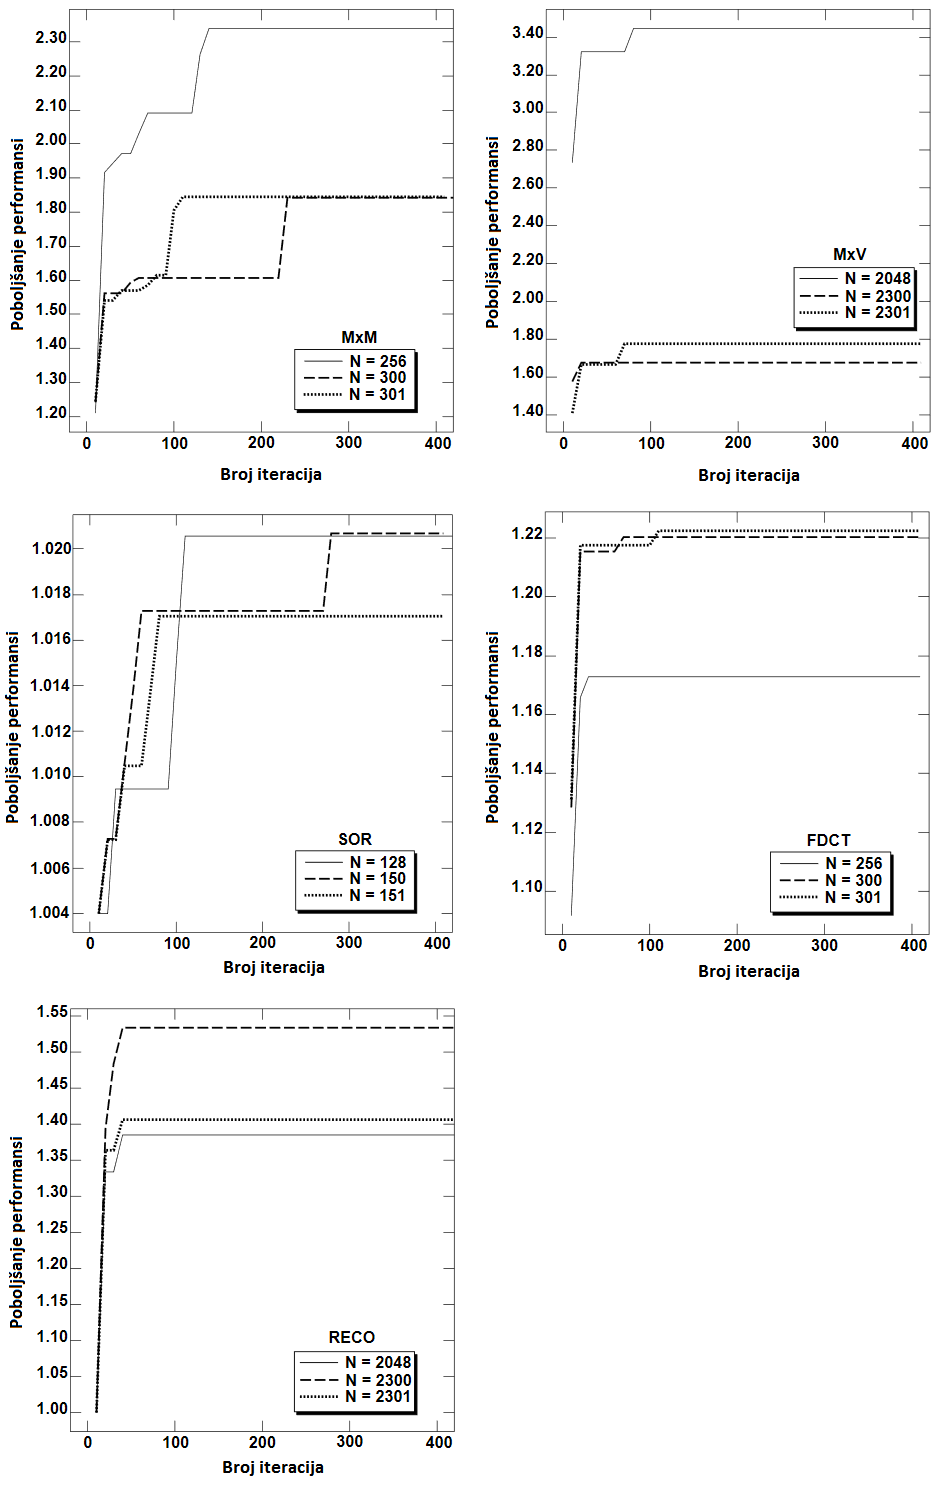
\includegraphics[width=\textwidth]{performanse1}
\end{center}
\caption{Poboljšanje performansi korišćenjem Odmotavanja i Podele na blokove}
\label{fig:slika1}
\end{figure}

\begin{figure}[p]
\begin{center}
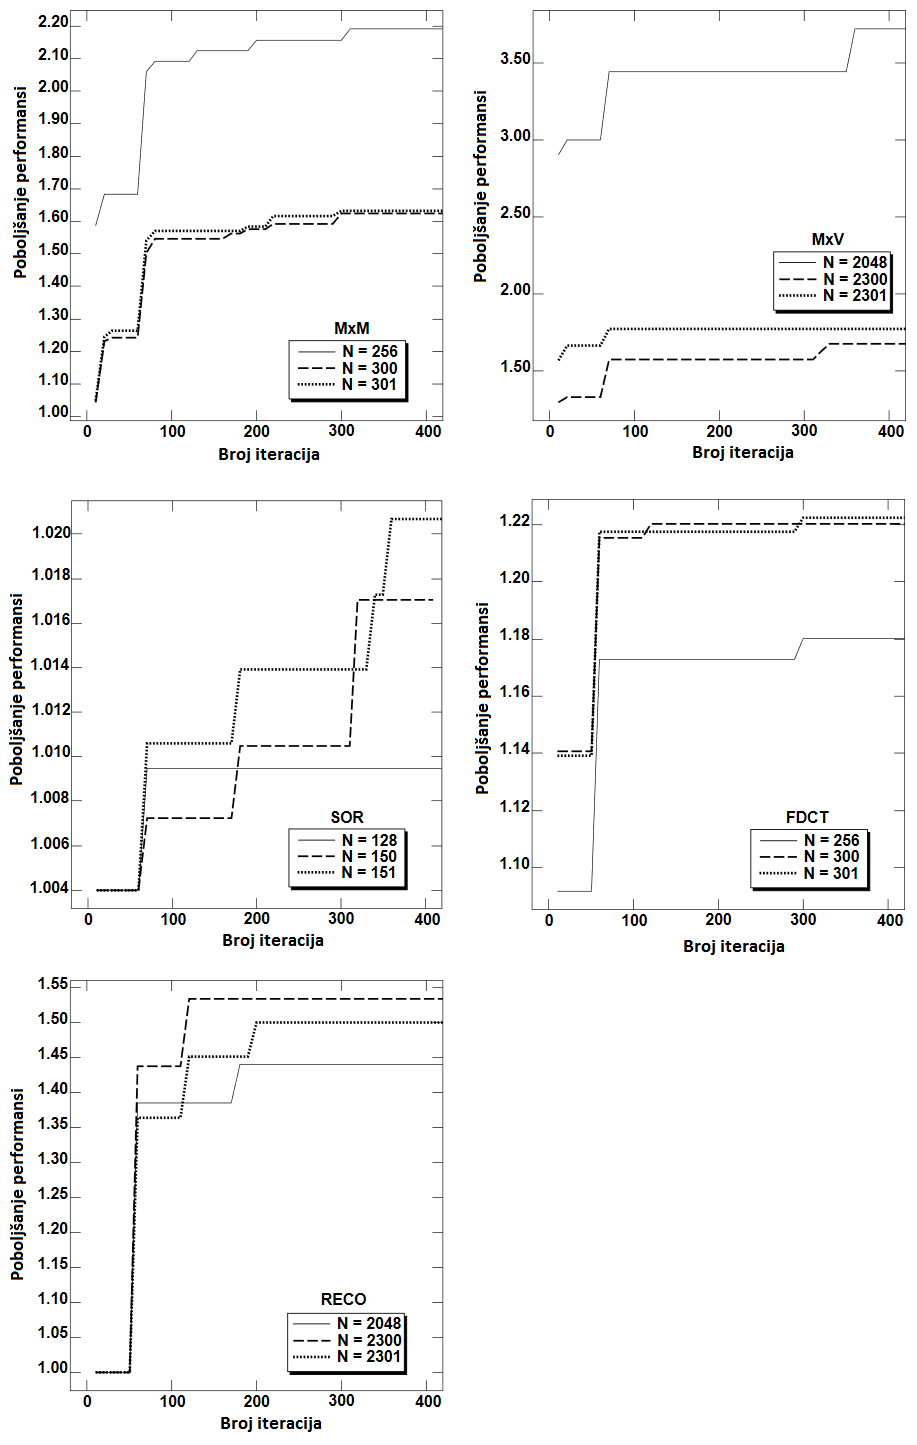
\includegraphics[width=\textwidth]{performanse2}
\end{center}
\caption{Poboljšanje performansi korišćenjem Odmotavanja, Podele na blokove i Array padding-a}
\label{fig:slika2}
\end{figure}


\section{Zaključak}
\label{sec:zakljucak}



\addcontentsline{toc}{section}{Literatura}
\appendix
\bibliography{seminarski} 
\bibliographystyle{plain}



\end{document}
